\documentclass[11pt]{article}
\usepackage[a4paper,margin=25mm]{geometry}
\usepackage[T1]{fontenc}
\usepackage{lmodern}
\usepackage{microtype}
\usepackage{booktabs}
\usepackage{graphicx}
\usepackage{caption}
\usepackage[hidelinks]{hyperref}
\captionsetup{font=small,labelfont=bf,width=.92\textwidth}
\setlength{\parskip}{0.6em}
\setlength{\parindent}{0pt}
\title{\textbf{Effect of ratio-band width on CT-HMM next-visit prediction}}
\date{5 November 2026}
\begin{document}
\maketitle
\thispagestyle{empty}

The ratio-band width in the next-visit CT-HMM was fixed at 0.1 by hand and never tested. This sweep tests four further widths either side of it. The width has an interior optimum near 0.3: narrower bands are worse, wider bands help up to 0.3, and at 0.5 every metric reverses. The gain over 0.1 is $+0.0026$ AUC, and it lies entirely outside the region of the ROC curve the model operates in.

\section*{Design}

Five main-range band widths plus the unbanded subtype-only model, over the same 934 leave-one-patient-out folds and the same 3,029 scored cases from 899 patients. Only the width changed: the three hidden states, the continuous-time generator, the interval-aware transition probabilities, the cohort, the emission floor and the seed are the published model's. The tail above ratio 3.0 is identical in every configuration -- the same ten bands, rebuilt inside each fold from the training patients alone -- so the comparison isolates the main range. All 5,604 fits converged and no fold failed.

\begin{table}[htbp]
\centering\small
\caption{Alphabet size and sparsity over the cohort's 4,295 labelled visits. Width 0.50 is the first configuration in which every category clears 30 observations.}\label{tab:complexity}
\begin{tabular}{lrrrrrrr}
\toprule
  \textbf{Width} & \textbf{Main bands} & \textbf{Categories} & \textbf{Params} & \textbf{Empty} & \textbf{Under 30 obs} & \textbf{Smallest} & \textbf{Obs/param} \\
\midrule
  0.05 & 60 & 73 & 224 & 11 & 40 & 1 & 19.2 \\
  0.10 & 30 & 44 & 137 & 1 & 12 & 1 & 31.4 \\
  0.20 & 15 & 29 & 92 & 0 & 2 & 8 & 46.7 \\
  0.30 & 10 & 24 & 77 & 1 & 2 & 8 & 55.8 \\
  0.50 & 6 & 20 & 65 & 0 & 0 & 35 & 66.1 \\
\bottomrule
\end{tabular}
\end{table}

\section*{Results}

Six of the seven metrics peak at width 0.30 -- accuracy, AUC-ROC, partial AUC, Brier score, log loss and calibration -- and PR-AUC peaks one step earlier, at 0.20. Whichever is taken as the summit, every metric falls back at 0.50, and the reversal is not selective: all seven move the wrong way together.

\begin{table}[htbp]
\centering\small
\caption{Held-out performance. Calibration is the mean absolute gap between predicted and observed P(PIGD) over the calibration bins; lower is better for it, for Brier and for log loss.}\label{tab:metrics}
\begin{tabular}{lrrrrrrr}
\toprule
  \textbf{Width} & \textbf{Accuracy} & \textbf{AUC-ROC} & \textbf{PR-AUC} & \textbf{Partial AUC} & \textbf{Brier} & \textbf{Log loss} & \textbf{Calib. gap} \\
\midrule
  no bands & 0.8369 & 0.8587 & 0.7496 & 0.7883 & 0.1214 & 0.3961 & 0.0065 \\
  0.05 & 0.8336 & 0.8739 & 0.7330 & 0.7802 & 0.1227 & 0.3952 & 0.0246 \\
  0.10 & 0.8316 & 0.8758 & 0.7398 & 0.7823 & 0.1221 & 0.3930 & 0.0283 \\
  0.20 & 0.8336 & 0.8775 & 0.7540 & 0.7868 & 0.1209 & 0.3898 & 0.0238 \\
  0.30 & 0.8359 & 0.8784 & 0.7523 & 0.7892 & 0.1199 & 0.3874 & 0.0222 \\
  0.50 & 0.8320 & 0.8765 & 0.7409 & 0.7827 & 0.1217 & 0.3916 & 0.0289 \\
\bottomrule
\end{tabular}
\end{table}

\begin{figure}[htbp]
\centering
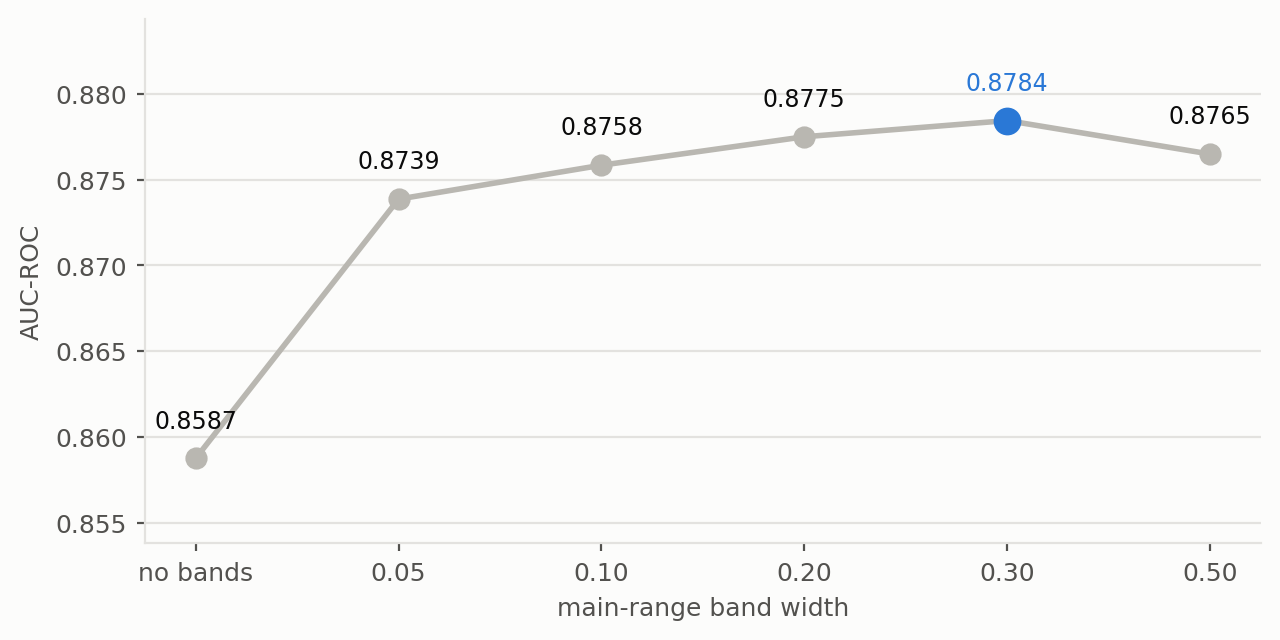
\includegraphics[width=0.86\textwidth]{figures/fig1_auc_by_width.png}
\caption{Discrimination peaks at band width 0.30 and then falls. Every width difference is small beside the difference between banding and not banding.}\label{fig:auc}
\end{figure}

\begin{table}[htbp]
\centering\small
\caption{Each configuration against the published 0.10 baseline, paired on patients, 2,000 bootstrap resamples. Width 0.30 excludes zero on all three; width 0.50 on none.}\label{tab:contrasts}
\begin{tabular}{lrlrrl}
\toprule
  \textbf{Width} & \textbf{AUC} & \textbf{95\% CI} & \textbf{PR-AUC} & \textbf{Partial AUC} & \textbf{95\% CI} \\
\midrule
  0.05 & $-0.0020$ & [$-0.0042$, $+0.0000$] & $-0.0068$ & $-0.0021$ & [$-0.0061$, $+0.0015$] \\
  0.20 & $+0.0017$ & [$-0.0002$, $+0.0036$] & $+0.0142$ & $+0.0045$ & [$+0.0010$, $+0.0082$] \\
  0.30 & $+0.0026$ & [$+0.0001$, $+0.0051$] & $+0.0125$ & $+0.0068$ & [$+0.0022$, $+0.0118$] \\
  0.50 & $+0.0006$ & [$-0.0023$, $+0.0036$] & $+0.0011$ & $+0.0003$ & [$-0.0066$, $+0.0068$] \\
\bottomrule
\end{tabular}
\end{table}

\section*{Why the sweep turns over}

The two subtypes want opposite things. TD owns the ten tail bands above ratio 3.0, which no main-range width touches, so TD only gains as main-range noise is stripped away and is at its best at the coarsest width tested. PIGD lives entirely below ratio 1.0, and widening from 0.30 to 0.50 cuts it from four categories to two: the positive class of the prediction target is the one whose resolution coarsening destroys.

\begin{figure}[htbp]
\centering
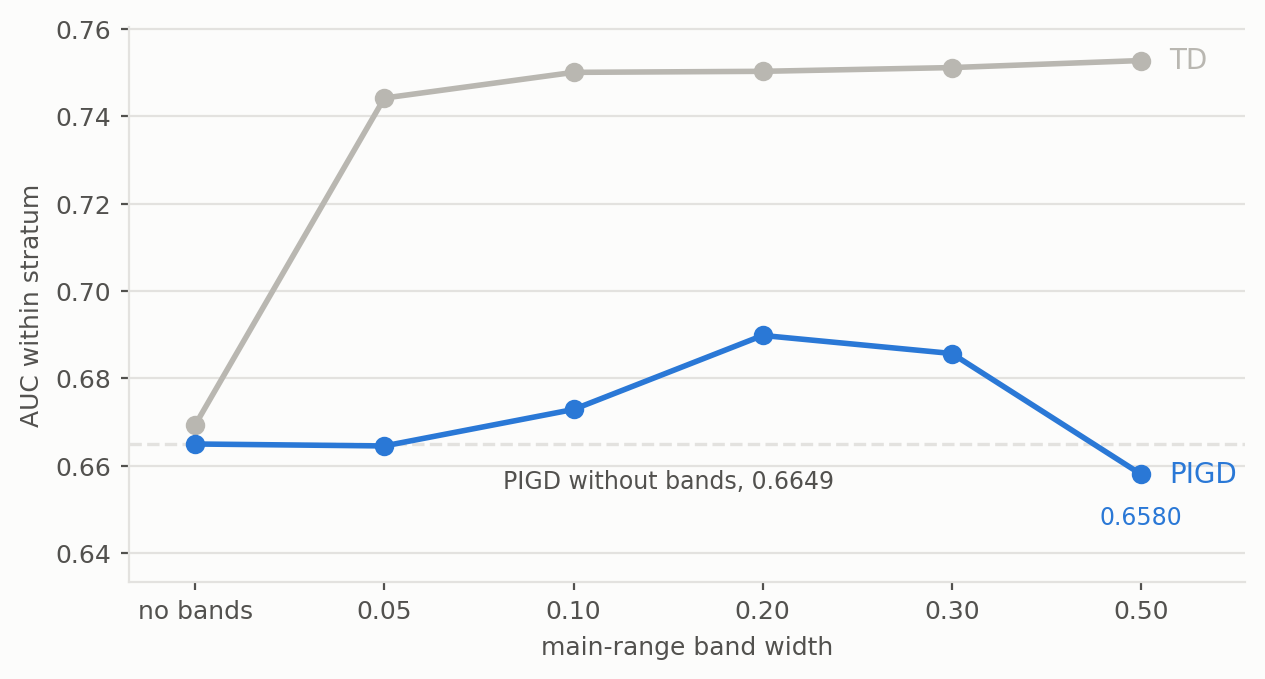
\includegraphics[width=0.86\textwidth]{figures/fig2_strata.png}
\caption{Within-stratum discrimination. At width 0.50 PIGD falls below the level it reaches with no bands at all, while TD is still improving.}\label{fig:strata}
\end{figure}

So the optimum near 0.3 is not a property of the ratio. It is the point where TD's preference for coarser bands and PIGD's need for finer ones balance, on this cohort and for this target. It also rules out the idea that the useful signal lies entirely in the tail: performance turns down well before the single-band limit. Sparsity is not the explanation either, since width 0.50 is the least sparse configuration in the study and among the worst performing.

\section*{Whether it matters clinically}

All six arms place their decision threshold at a false-positive rate between 0.09 and 0.12. Restricting the comparison to that end of the curve -- McClish-standardised partial AUC at FPR $\le$ 0.2 -- every width's advantage over no banding disappears, the optimum included.

\begin{figure}[htbp]
\centering
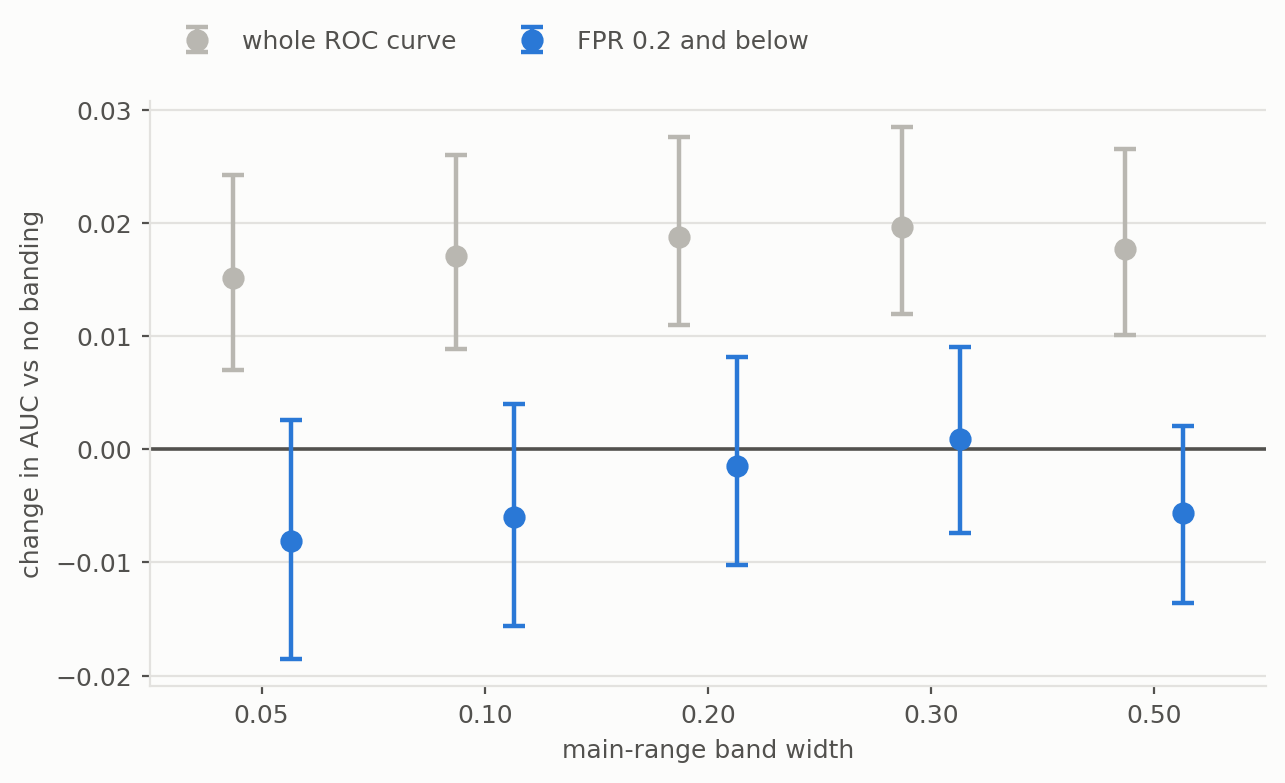
\includegraphics[width=0.86\textwidth]{figures/fig3_contrasts.png}
\caption{Each width against no banding. Over the whole curve every interval clears zero; in the usable region every interval crosses it.}\label{fig:contrasts}
\end{figure}

\begin{table}[htbp]
\centering\small
\caption{Secondary contrasts against the unbanded model. Added after the primary analysis and refitting nothing, so they are descriptive rather than confirmatory.}\label{tab:secondary}
\begin{tabular}{lrlrrl}
\toprule
  \textbf{Width} & \textbf{AUC} & \textbf{95\% CI} & \textbf{PR-AUC} & \textbf{Partial AUC} & \textbf{95\% CI} \\
\midrule
  0.05 & $+0.0151$ & [$+0.0070$, $+0.0243$] & $-0.0166$ & $-0.0081$ & [$-0.0186$, $+0.0026$] \\
  0.10 & $+0.0171$ & [$+0.0089$, $+0.0260$] & $-0.0098$ & $-0.0060$ & [$-0.0156$, $+0.0040$] \\
  0.20 & $+0.0188$ & [$+0.0110$, $+0.0276$] & $+0.0044$ & $-0.0015$ & [$-0.0102$, $+0.0081$] \\
  0.30 & $+0.0197$ & [$+0.0120$, $+0.0285$] & $+0.0027$ & $+0.0009$ & [$-0.0074$, $+0.0090$] \\
  0.50 & $+0.0177$ & [$+0.0101$, $+0.0265$] & $-0.0087$ & $-0.0057$ & [$-0.0136$, $+0.0021$] \\
\bottomrule
\end{tabular}
\end{table}

Banding costs calibration at every width. The unbanded model's mean absolute calibration gap is 0.0065; the best banded arm is 0.0222 and the worst, width 0.50, is 0.0289. No width improves next-visit accuracy either: every accuracy interval in the study includes zero, and the unbanded model still scores highest at 0.8369.

\section*{Conclusion}

Going below 0.1 makes things worse: width 0.05 spends 224 parameters on 73 categories, 40 of them holding fewer than 30 observations, and is never the best arm on anything. Going above helps to about 0.3 and then reverses. The band width was not what held the previous experiment back.

If the banded model is kept, 0.30 is the width to keep -- best on six of seven metrics and, at 77 parameters, nearly the simplest. But the optimum buys a third decimal place of AUC in a region of the curve nobody operates in, while costing a factor of three in calibration. That is the finding to report, not a recommendation to change the model.

\section*{What this does not support}

\begin{itemize}
  \item It is partly post hoc. Four widths were pre-specified; 0.50 was added after seeing that the trend had not turned over, and the contrasts against no banding were added after the primary analysis. Both refit nothing, and the pre-specified results are unchanged.
  \item Naming a winner is selection on the evaluation set, so the winner's held-out numbers are optimistically biased. Width was never tuned against held-out performance inside the fits.
  \item The peak is bracketed only coarsely. Near 0.3 is supported; exactly 0.30 is not, and the falling limb rests on a single point.
  \item A confound remains: the subtype thresholds fall on the band grid at some widths and not others, so the number of bands a threshold cuts through runs 1, 2, 2, 1, 2 and is not monotone in the width.
  \item One cohort, one frozen panel, one prediction target, no external validation.
\end{itemize}

\end{document}
